%preamble
\documentclass[letterpaper]{article}
\synctex=1
\usepackage{graphicx}
\graphicspath{ {images/} }

\usepackage{lipsum}

%actual document
\begin{document}

  % \maketitle %insert titlepage here
  \begin{titlepage}
    \begin{center}
        \vspace*{1cm}
        \Huge
        Experiment 2
        \vspace{1cm}

        Electostatic Potentials and Fields
        \vspace{1cm}

        By: Arun Woosaree
        \vspace{1cm}

        Lab partners:

        \vspace{1cm}
        \Large
        NameMcNameface
        \vspace{1cm}

        \Huge
        PHYS 230 Lab EH71
        \vspace{1cm}

        TA: The Worst Physics TA Ever
        \vspace{1cm}

        Date of Lab: \today
        \vfill
    \end{center}
\end{titlepage}

\section{Introduction}
In experiment 8, we explore the conservation of energy, specifically the transformation of potential energy into kinetic energy, and also the conversion of kinetic energy into potential energy using a mass hanging on a pendulum, and a spark-tape record. In the beginning, the bob is held at a height with some potential energy and is released from rest (meaning zero kinetic energy). Naturally, the bob starts moving due to gravity, which means the bob’s potential energy is being turned into kinetic energy. The reverse also happens after the bob has reached its lowest height relative to the ground as it oscillates. After that point, kinetic energy is converted back into potential energy.
The kinetic energy of any object with mass m can be determined with the formula
Where ‘EK’ is the kinetic energy, ‘m’ is the mass of the object, and ‘v’ is the velocity of the object.
For the pendulum,  where ‘r’ is the length of the string of the pendulum to the center of the bob, ‘R’ is the length of the string to the spark track, and ‘V’ is the instantaneous velocity of the bob. ‘V’ can be approximated as: , where ‘ΔS’ is the change in displacement of the bob during a small length of time ‘Δt’ (due to Δt being small). At a spark number ‘n’,  where ‘sn+1’ is the displacement of the bob after spark n and ‘sn-1’ is the displacement of the bob before spark n.  The displacements are measured with respect to where the bob hangs at rest at the center of the pendulum. Subsequently, ‘tn+1’ is the time when the spark after spark ‘n’ was made, and ‘tn-1’ is the time before spark n. The equations can be put together to get:



The potential energy of any object with mass m can be found using the equation
Where ‘Ep’ is the gravitational potential energy of the object, ‘g’ is the acceleration due to gravity on Earth, and ‘h’ is the height of the object. For the pendulum, h is the height of the bob with respect to the lowest point at the center of the pendulum, which can be found using the following formula:
. Recall that ‘r’ is the length of the string of the pendulum to the center of the bob. ‘θ’ can be found using  where ‘θ’ is expressed in radians. Recall that ‘S’ is the displacement of the bob and ‘R’ is the length of the string to the spark track.  The equations can be combined to get:


The total energy, (ET) of the bob is  , because of the law of conservation of energy which says that energy cannot be created or destroyed, but can be converted. We can expect ET to be constant, assuming no energy loss due to things like friction, since at the highest position, the bob has all potential energy, at the lowest position, all of its potential energy (ideally) is converted into kinetic energy, and as the bob rises to the top again, its kinetic energy is stored once again as potential energy. We can see scenarios akin to this that are pretty common in real life, such as in rollercoasters.  For rollercoasters, there is always the part where the car moves slowly at a steep incline. This is where gravitational potential energy is being stored as the car rises. This potential is then converted into kinetic energy as the car drops down, and speeds up due to the increase in kinetic energy. The kinetic energy is then converted back into gravitational potential energy when the car goes up again, and slows down, possibly due to going in a loop, where the conversion of kinetic energy and potential energy continue onwards.
On a graph with ET , EP , and EK  as functions of time (total time is half a period in this experiment), we would expect to see ET ­ as a horizontal, constant line, with EP initially being the same value as ET ,and EK being zero. About halfway, we would expect EP to be zero, and EK=ET because all of the potential energy should theoretically have converted into kinetic energy at that point. Finally, at the end of the graph we expect all of EK­ to have converted back into EP. (Hence, EK=0 , EP = EK)

  \begin{equation}
    F_e=\frac{k q_1 q_2}{r^2}
  \end{equation}

  \begin{equation}
    F_e \cos\theta - F_g \sin\theta=0
  \end{equation}

  \begin{equation}
    \frac{F_e}{F_g} = \tan\theta
  \end{equation}

  \begin{equation}
    \frac{d_1}{l}=\sin\theta
  \end{equation}

  \begin{equation}
    F_e=F_g\frac{d_1}{l}
  \end{equation}

  \begin{equation}
    \frac{k q_1 q_2}{r^2}=mg\frac{d_1}{l}
  \end{equation}

  \begin{equation}
    \frac{h}{H}=\frac{r}{R}=\frac{d_1}{D_1}=\frac{d_2}{D_2}
  \end{equation}

  \begin{equation}
    D_1=(\frac{H}{h})^3 (\frac{l}{mg}) \frac{k q_1 q_2}{R^2}
  \end{equation}

\section{Experimental Method}

\begin{figure}[h!]
    \centering
    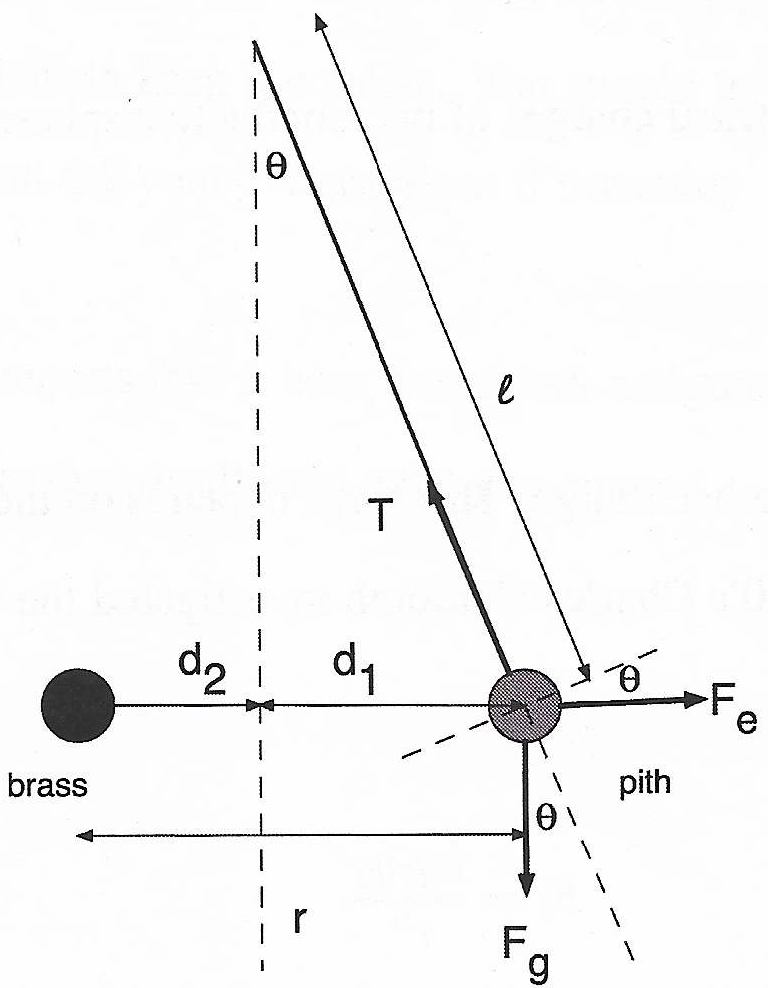
\includegraphics[width=0.4\textwidth]{fig1crop.png}
    \caption{Forces acting on the charged pith ball}
\end{figure}

\begin{figure}[h!]
    \centering
    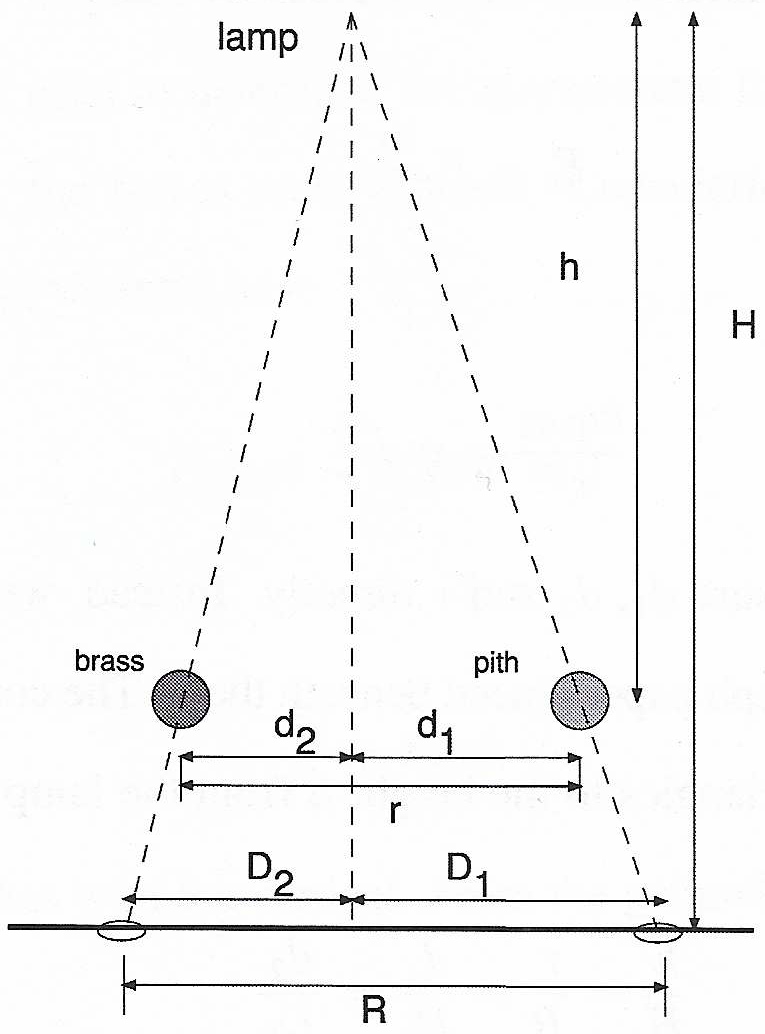
\includegraphics[width=0.4\textwidth]{fig2crop.png}
    \caption{The separation between the balls in relation to the separation between their shadows}
\end{figure}

When the apparatus illustrated above is set up, i.e. the lengths ‘r’ and ‘R’ are known, the center of the spark tape is marked when the bob is hanging freely at rest, and the bob is at the starting position, being held by the electromagnet, and the string is steadied to lessen any vibrations, the power going to the electromagnet is cut, and as a result, the bob is released from rest. The ‘RUN’ button on the spark timer is immediately (as best as humanly possible) held down, until the bob reaches approximately the maximum height on the other side of the track, or when one half of the period of the pendulum is completed.

The spark timer is set to spark 30 times a second, so the time elapsed between each burn hole on the spark tape is 1/30th of a second. Once the spark tape is obtained from the apparatus, we need to measure the displacements of the glider as it was moving. To do so, we use a meter stick, and a displacement of 0.00m is taken to be the at the center of the spark tape, which is the point that was marked while the bob hangs freely at rest. This means that the initial displacement of the bob is taken to be a negative displacement, and the points after the bob passes the center are taken to be positive.

After measuring the displacements of the bob, we enter the data points into Excel, and also calculate the time elapsed for each data point. (Ex. At the 10th burn hole, the time elapsed would be 10*1/30 seconds). From this data, we can calculate EK , EP , and ET  using equations  5,9 and 10 and plot them on a graph as a function of time. The ET curve was fit to a linear regression, and the EK and EP curves were fit to quadratic curves.

\section{Results}
  \lipsum[3]

\section{Discussion}
The results from the lab overall seemed reasonable, because the data fit pretty nicely to the curves that we expected them to in the graph. ET was fit to a linear curve, and EK and EP were fit to quadratic curves.  (Fig.2).  The value calculated for energy loss per second from the graph (-0.44739±0.510812 J/s) does not agree within error of the expected value we calculated (0.00161 J/s) which was calculated by measuring the initial and final displacement of the bob on the pendulum after 25 periods, finding the initial and final potential energies, calculating the total time for 25 periods, and then finding the average energy loss per second. The calculated value from the graph is 3 orders of magnitude different. However, given that the slope of the graph(fig.4) seemed almost flat, the data still seems somewhat reasonable.

We did, however have to omit 4 anomalous data points from the curve fits, because it is very unlikely that the bob was moving about 12 or 25 m/s at any point along the track. These anomalous data points can be attributed to the spark timer missing two sparks, since one missing spark would significantly impact two data points for the instantaneous velocity, since the bob would appear to move a lot faster than it actually did for two data points. It appears to move faster since the instantaneous velocity is calculated using the data points from before and after spark n, and a missing spark in the data makes it seem that the bob is moving a greater distance in a shorter time than it actually is. (see eq. 4). Two missing sparks would have caused four calculated instantaneous velocities to be significantly higher than they should be, and since instantaneous velocity is used to calculate EK on the graph, EK at the two points where the spark was missed would be significantly higher than they should be. Once can even see on the graph that the four anomalous data points are in pairs of two. (One at 20-25 J and the other at 10-15 J). Because ET includes EK, there are four anomalous data points for ET as well, at the exact same time.  Hence, these data points were ignored when fitting curves to the data.

On the graph (fig.4), we would expect to see ET as a constant, horizontal line, and indeed, the linear fit seems to be almost horizontal. The line is not horizontal, however, and it has a slight downwards slope of -0.44739±0.510812 J/s . This is due to the loss of energy. In an ideal scenario, with no energy loss, the line should be perfectly flat, however energy was being lost due to factors such as air friction, friction with the bob on the track, and vibrations on the string. At t=0, we see that ET and EK are almost the same values, as we would expect since at the beginning, the bob is not moving, so EK would be zero. (Also confirmed on the graph.) As the bob is moving down, we would expect EP to be converted into EK, and we see that on the graph, EP is decreasing as EK increases, up until EP is about 0 and EK is almost equal to ET, which is definitely observed on the graph. After that point, one would expect, and can also see on the graph that EK would be converted back into EP, until EK is almost 0, and EP is about ET. This data agrees with the law of conservation of energy, as we can visually see from the graph what types of energy are being converted, whilst observing the total energy being almost constant. (Since we are not working in an ideal scenario, and energy is lost due to factors such as friction.)

\section{Conclusions}
  In lab 8, we set up a pendulum with a 2.3kg bob hanging off of a string, and put an arced track such that the bob would be close enough to the track at any point while it swings to make a spark, with a spark timer. We then used an electromagnet to release the bob from rest, and used the spark timer to keep track of the bob’s displacements, and since the spark timer sparks at regular intervals, we had enough data to generate plots in Excel of potential energy, kinetic energy, and total energy as functions of time. The law of conservation of energy says that energy cannot be created or destroyed, but it can be converted. Theoretically, all of the Pe at the beginning should convert completely into KE, and then towards the end, all of the KE that the bob has should convert back into PE. Indeed, we do observe this behaviour in the lab, albeit not perfectly, since energy is also lost due to some of it being converted to other forms such as friction. This caused TE to decrease over time. Additionally, there were some anomalous data points that can be attributed to the spark timer missing sparks. Overall, however, the data seemed reasonable, albeit the amount of energy lost per second using the graph’s data versus taking an average after 25 periods did seem to disagree with 3 orders of magnitude.  One can observe the physics principles explored in the lab in real-life such as on a rollercoaster, where the gravitational potential energy is also converted into kinetic energy and vice versa such as when the car is going through a loop.

\end{document}
